\documentclass[a2paper, 12pt]{article}
\usepackage[font={huge, bf}]{caption}
\usepackage{fontspec}
\setmainfont{Arial}
\usepackage{subcaption}
\usepackage{graphicx}
\usepackage{tikz}
\usepackage{tikzsymbols}
\usetikzlibrary{calc,patterns,shapes.geometric}
\usepackage{float}
\usepackage{pdflscape}
\usepackage{geometry}
\geometry{landscape, margin=2cm}
\captionsetup[subfigure]{justification=justified,singlelinecheck=false}
\pagestyle{empty}

\def\centerarc[#1](#2)(#3:#4:#5){\draw[#1] ($(#2)+({#5*cos(#3)},{#5*sin(#3)})$) arc (#3:#4:#5);}

\begin{document}
	\vspace*{\fill}
	\begin{figure}[!htbp]
		\centering
		\begin{subfigure}[b]{0.48\textwidth}
			\caption{Figure 1}
			\centering
			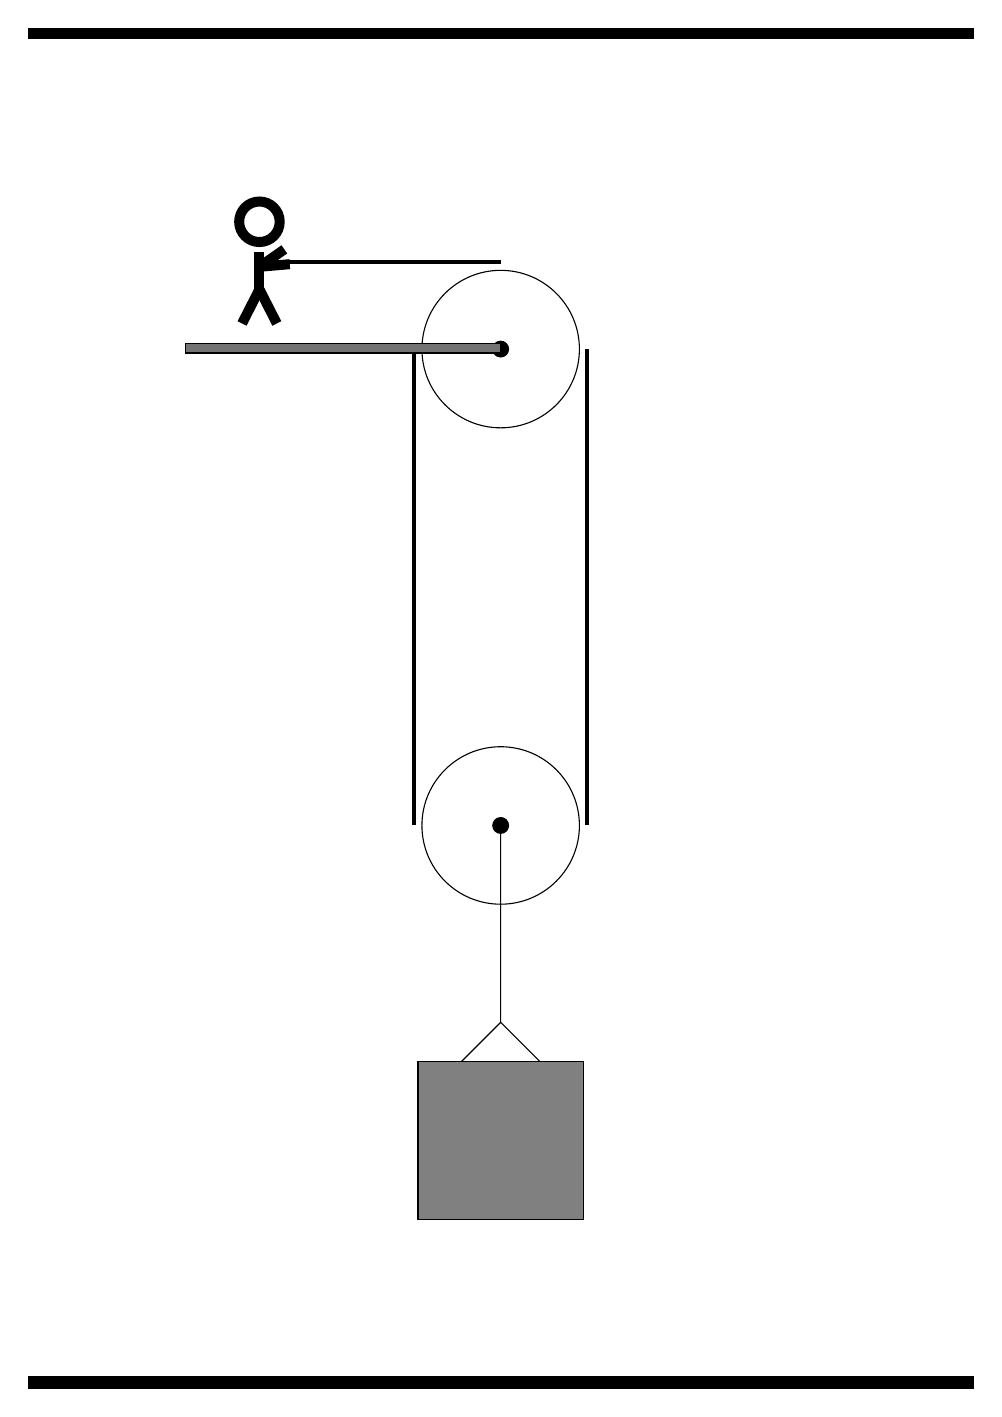
\begin{tikzpicture}
				\draw[fill=black] (-4, 14) rectangle (8, 14.125);
				
				\draw (2, 4.0) circle (1);
				\draw[fill=black] (2, 4.0) circle (0.1);
				
				\draw (2, 10.05) circle (1);
				\draw[fill=black] (2, 10.05) circle (0.1);
				
				\draw (2, 4.0) -- (2, 1.5) -- (1.5, 1.0) -- (2.5, 1.0) -- (2, 1.5);
				\draw[fill=black!50] (0.95, 1.0) rectangle (3.05, -1.0);
				
				\draw[line width=0.5mm] (0.9, 10) -- (0.9, 4.0);
				\centerarc[line width=0.5mm](2, 4.0)(180:360:1.1);
				\draw[line width=0.5mm](3.1, 4.0) -- (3.1, 10.05);
				\centerarc[line width=0.5mm](2, 10.05)(0:90:1.1);
				\draw[line width=0.5mm](2, 11.15) -- (-1, 11.15);
				
				\node at (-1, 11.15) {\scriptsize \Strichmaxerl[10][-175][35]};
				\draw[fill=black!55] (-2, 10) rectangle (2, 10.125);
				
				\draw[fill=black] (-4, -3) rectangle (8, -3.15);
			\end{tikzpicture}
		\end{subfigure}
		\hfill
		\begin{subfigure}[b]{0.48\textwidth}
			\caption{Figure 2}
			\centering
			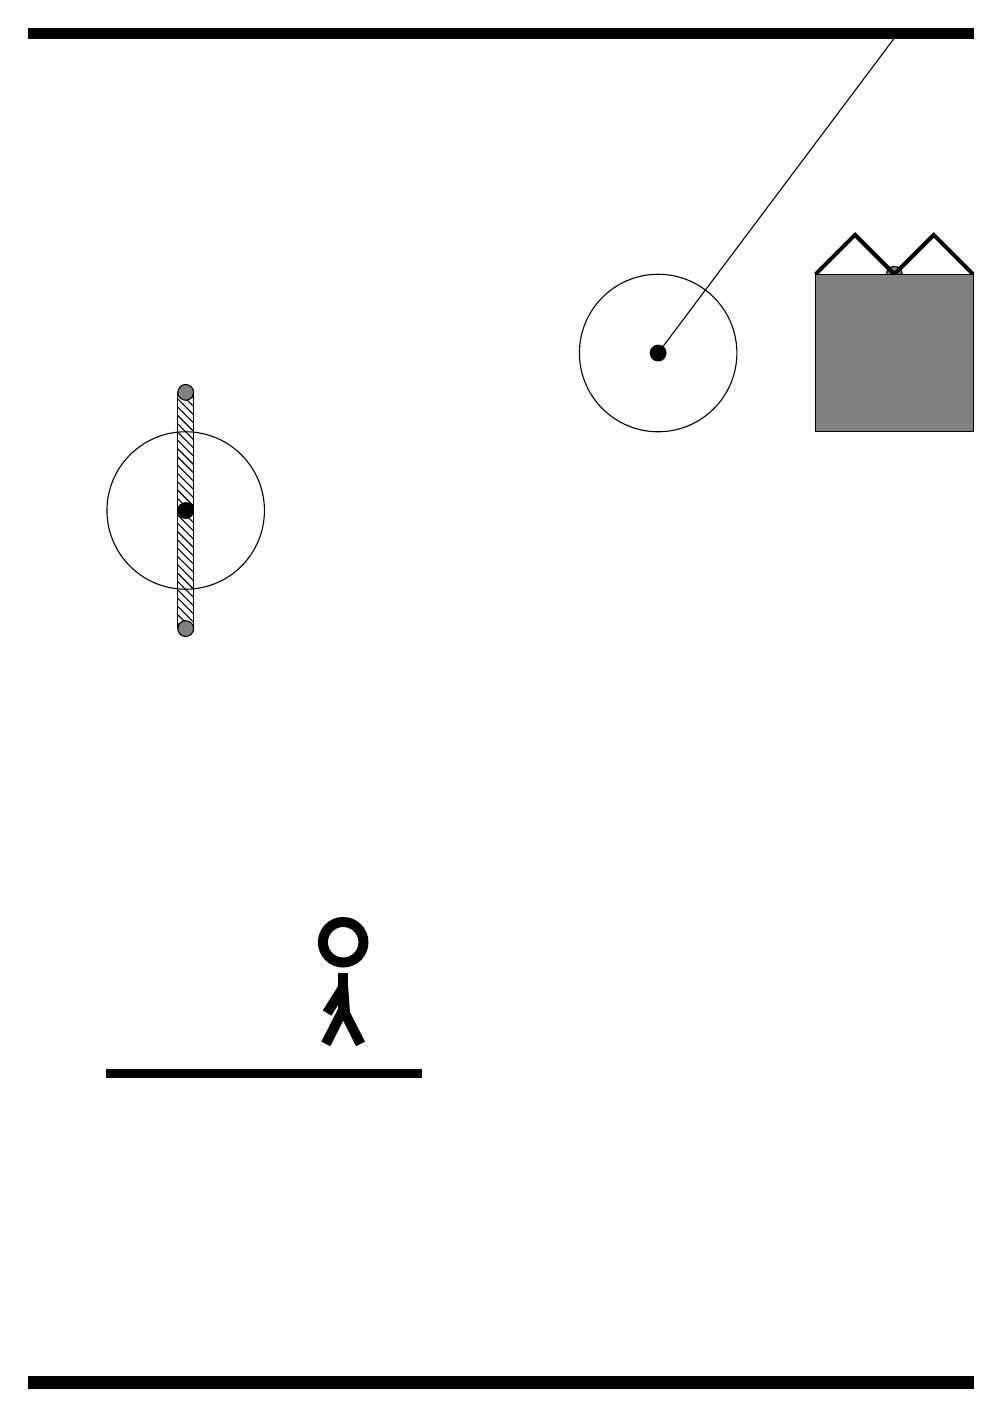
\begin{tikzpicture}
				\draw[fill=black] (-4, 14) rectangle (8, 14.125);
				
				\draw (4,10) circle (1);
				\draw[fill=black] (4,10) circle (0.1);
				\draw (7,14.0) -- (4,10);
				
				\draw (-2,8) circle (1);
				\draw[fill=black] (-2,8) circle (0.1);
				\draw[pattern=north west lines, pattern color=black] (-2.1,9.5) rectangle (-1.9,6.5);
				\draw[fill=black!50] (-2,9.5) circle (0.1);
				\draw[fill=black!50] (-2,6.5) circle (0.1);
				
				\draw[fill=black!50] (7,11) circle (0.1);
				\draw[line width=0.5mm](6.5,11.5) -- (7,11) --  (7.5,11.5);
				\draw[line width=0.5mm](6,11) --  (6.5,11.5) -- (7,11) -- (7.5,11.5) -- (8,11);
				\draw[fill=black!50] (6, 11) rectangle (8, 9);
				
				\node at (0, 2) {\scriptsize \Strichmaxerl[10][94][-122]};
				\draw[fill=black] (-3, 0.8999999999999999) rectangle (1, 0.8);
				
				\draw[fill=black] (-4, -3) rectangle (8, -3.15);
			\end{tikzpicture}
		\end{subfigure}
	\end{figure}
		\vspace*{\fill}
\end{document}